\documentclass[a4paper,12pt,fleqn]{article}%fleqn pour aligner les equations à gauche
\usepackage{../../Styles/Cours}


\newcommand{\chnum}{Chapitre 1}
\newcommand{\chtitle}{A la découverte de la spectrophotométrie !}
\newcommand{\dtype}{\\Activité 1}

\begin{document}
	\maketitle
	
	\begin{figure}[h!]
		\caption{Couleur d'une solution}
		\label{doc1}
		\begin{minipage}{.48\linewidth}
			Lorsqu'une solution est traversée par de la lumière blanche, certaines radiations sont absorbées et d'autres sont transmises.\\
			La couleur perçue d'une solution est complémentaire des radiations absorbées par le trajet dans la solution. Les couleurs complémentaires sont diamétralement opposées sur le cercle chromatique.\\
			\emph{Plus la concentration d'une espèce colorée en solution est élevée, plus les radiations sont absorbées et plus la solution est foncée.}
		\end{minipage}
		\begin{minipage}{.48\linewidth}
			\centering 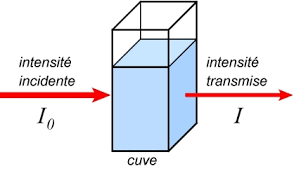
\includegraphics[scale=.75]{Ressources/1SPE_C1_Act1_Fig1.png}\\
			\textbf{A}
		\end{minipage}
		
		\begin{minipage}{.48\linewidth}
			\centering 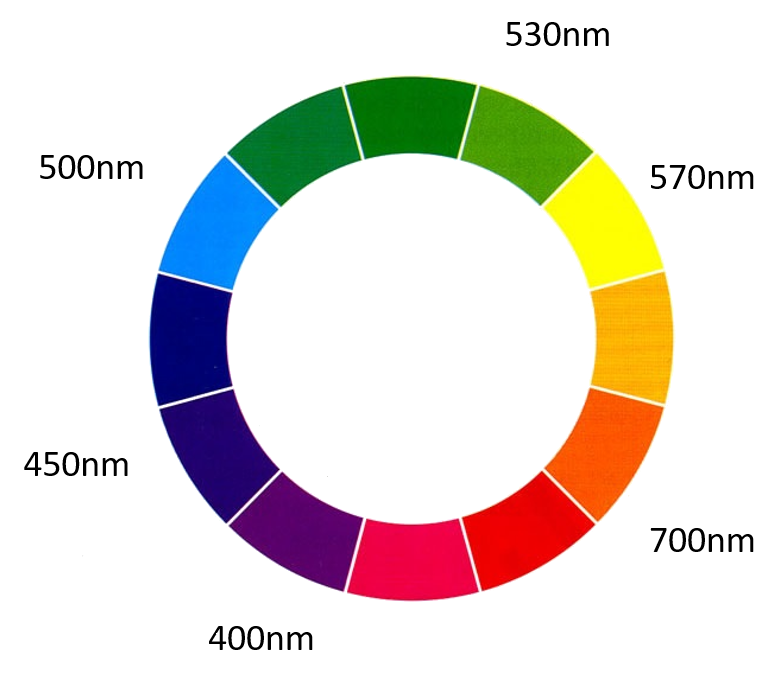
\includegraphics[height=6cm]{Ressources/Cercle_chromatique.png}\\
			\textbf{B}
		\end{minipage}
		\begin{minipage}{.48\linewidth}
			\centering 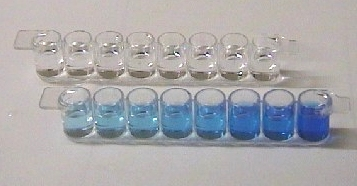
\includegraphics[height=5cm]{Ressources/1SPE_C1_Act1_Fig3.jpg}\\
			\textbf{C}
		\end{minipage}
	\end{figure}
	
	\begin{figure}[h!]
		\caption{Couleur d'une solution et absorbance}
		\label{doc2}
		\begin{minipage}{.48\linewidth}
			Pour une longueur d'onde donnée, l'absorbance $A$ quantifie la proportion des radiations incidentes notées $I_0$ absorbées en mesurant l'intensité des radiations non absorbées $I$. Pour une espèce chimique donnée, la courbe $A=f(\lambda)$ est appelée un spectre d'absorption. Elle permet de déterminer la longueur d'onde de l'absorbance maximale que l'on note $\lambda_{max}$. Cette longueur d'onde correspond à la couleur complémentaire de celle de la solution.
		\end{minipage}
		\begin{minipage}{.48\linewidth}
			\centering 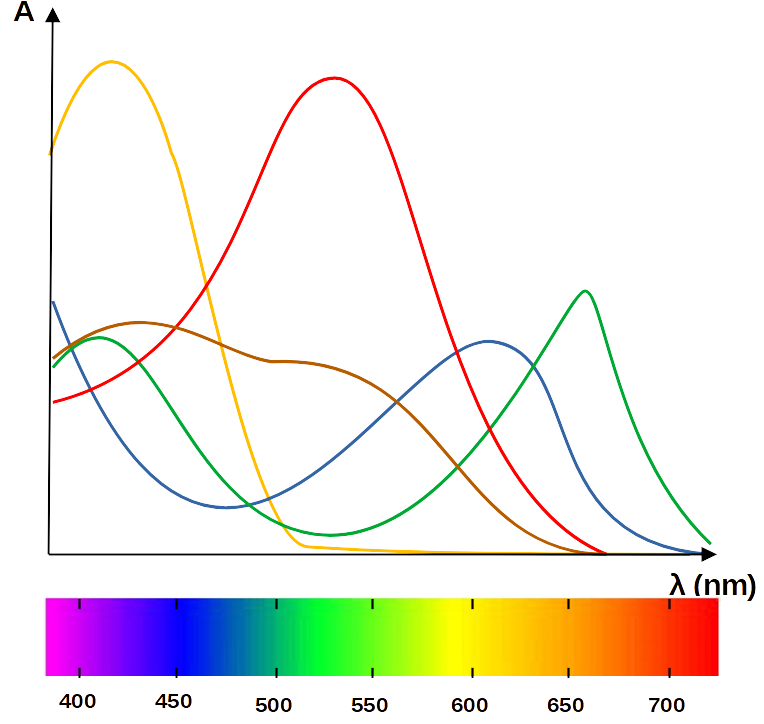
\includegraphics[height=9cm]{Ressources/Spectre_absorption.png}
		\end{minipage}
	\end{figure}
	
	\begin{figure}[h!]
		\caption{Dosage spectrophotométrique par étalonnage}
		\label{doc3}
		Pour une longueur d'onde $\lambda$ donnée, l'absorbance $A_\lambda$ d'une solution est proportionnelle à la concentration en soluté coloré de celle-ci. Il est donc possible de relier ces deux grandeurs grâce à une \emph{courbe d'étalonnage}, si toutes les mesures dont faites avec une cuve de même largeur (appelée trajet optique).\\
		Selon la loi de Beer-Lambert; l'absorbance d'un soluté a une longueur d'onde donnée notée $A_\lambda$ et la concentration en soluté $C$ sont proportionnelles et répondent à la relation suivante :\\
		\begin{tabular}{>{\centering} m{4cm}|m{14cm}}
			
			\multirow{4}{*}{$A_\lambda = \epsilon \cdot l \cdot C$} & $A_\lambda$ : l'absorbance de la solution mesurée à la longueur d'onde $\lambda$, sans unité\\
			& $\epsilon_\lambda$ : le coefficient d'extinction molaire, propre à une espèce chimique pour une longueur d'onde donnée, en \unit{\liter \per\mole\per\centi\meter}\\
			& $l$ : le trajet optique en \unit{\centi\meter}\\
			& $C$ : la concentration molaire en soluté coloré, en \unit{\mole\per\liter}\\
		\end{tabular}
				
		Il est possible d'accéder expérimentalement à la valeur de $\epsilon_\lambda$ en traçant la courbe $A_\lambda = f(C)$. pour des concentrations faibles, cette courbe sera une droite dont le coefficient directeur aura pour valeur $k=\epsilon_\lambda \cdot l$.
	\end{figure}
	\begin{figure}[h!]
		\caption{Questions :}
		\begin{enumerate}
			\item Quelle est la couleur de la radiation absorbée par la solution présentée sur la figure \textbf{C} (Doc.~\ref{doc1}) ?
			\item Décrire la figure \textbf{C} en termes d'intensité de radiation absorbée" et de "concentration molaire en soluté". (Doc.~\ref{doc1})
			\item Préciser pour chacune des couleurs de solutions représentées, à quelle longueur d'onde correspond le maximum d'absorbance de la solution (Doc.~\ref{doc2})
			\item Justifier pour chacun des cas précédents la couleur de la solution. Quelle est la particularité de la solution verte ? (Doc.~\ref{doc1} et~\ref{doc2})
			\item Selon vous pour la solution rouge, quelle est la portion d'onde à choisir pour obtenir une mesure d'absorbance la plus précise possible ? (Doc.~\ref{doc1} et~\ref{doc2})
			\item En quoi la loi de Beer-Lambert est en accord avec la portion soulignée du Doc.~\ref{doc1} ? Quelles informations supplémentaires cette loi apporte-t-elle ? (Doc.~\ref{doc1} et~\ref{doc3})
			\item En se basant sur l'ensemble des documents, élaborer une stratégie pour déterminer la concentration d'ions cuivre \RNum{2} contenu dans une solution d'absorption $A_{\ce{Cu^{2+}}}  = 0.85$.
		\end{enumerate}
	\end{figure}
	
\end{document}